\chapter{System Requirements and Concept}

\section{System Objectives}

The primary objective of the developed system is to provide an accessible,
browser-based virtual laboratory for interactive physics experiments. The
laboratory should be usable without requiring dedicated native software and
should support both conventional desktop computers and standalone VR headsets,
such as the Meta Quest 3, through compatible web browsers.

A second objective is to provide an immersive and interactive representation
of physics experiments. Users should be able to manipulate virtual experimental
equipment and observe the resulting behaviour within the three-dimensional
environment. The implemented experiments cover different areas of physics,
including geometrical optics through the Convex Lens experiment and quantum
physics through the Stern--Gerlach experiment.

The system is also intended to support collaborative experimentation. Multiple
users should be able to enter the same virtual laboratory, observe one another
through avatar representations, interact with synchronized experimental objects
and states, and communicate verbally within the shared environment. Changes
made by one participant should be communicated consistently to the other
participants in the same session.

Another objective is to provide a common interaction model across the supported
platforms. Users should be able to navigate the laboratory and interact with
experimental equipment using either VR controllers or conventional desktop
input devices.

The laboratory is designed with a modular structure so that additional physics
experiments can be integrated without requiring fundamental changes to the
underlying navigation, WebXR, multiplayer, and communication infrastructure.
The system is also intended to remain deployable using standard web
technologies, allowing the complete laboratory to be accessed through modern
WebXR-compatible browsers.

\section{Functional Requirements}

Based on the system objectives defined in Section~3.1, the following functional
requirements were specified for the virtual laboratory.

\renewcommand{\arraystretch}{1.3}
\begin{longtable}{p{2cm} p{12cm}}
\caption{Functional requirements of the proposed virtual laboratory system}
\label{tab:functional_requirements} \\
\hline
\textbf{ID} & \textbf{Requirement} \\
\hline
\endfirsthead

\hline
\textbf{ID} & \textbf{Requirement} \\
\hline
\endhead

FR-01 &
The system shall be accessible through a compatible web browser without
requiring the installation of dedicated native software. \\
\hline

FR-02 &
The system shall support both conventional desktop access and immersive
Virtual Reality access through WebXR-compatible headsets. \\
\hline

FR-03 &
The system shall provide a virtual laboratory containing multiple rooms and
at least two interactive physics experiments representing different areas of
physics. \\
\hline

FR-04 &
Users shall be able to navigate through the virtual laboratory and move
between the available laboratory areas. \\
\hline

FR-05 &
Users shall be able to interact with virtual experimental equipment using VR
controllers or conventional desktop input devices. \\
\hline

FR-06 &
The system shall provide interactive experiment behaviour in which user
actions modify relevant experiment parameters and produce corresponding
visual or numerical results. \\
\hline

FR-07 &
The system shall allow multiple users to connect concurrently to the same
virtual laboratory session. \\
\hline

FR-08 &
The system shall synchronize relevant user, interactive-object, and
experiment states between participants in the same session. \\
\hline

FR-09 &
Connected users shall be represented within the shared virtual environment
using avatars or equivalent visual representations. \\
\hline

FR-10 &
The system shall support real-time voice communication between connected
participants within the shared virtual environment. \\
\hline

FR-11 &
Changes made to shared interactive objects by one participant shall be
visible to the other participants in the same session. \\
\hline

FR-12 &
The system shall maintain a consistent experiment state for connected
participants during collaborative interaction. \\
\hline

FR-13 &
The system shall support the integration of additional physics experiments
without requiring fundamental changes to the common navigation, WebXR,
multiplayer, and communication infrastructure. \\
\hline

FR-14 &
Users who disconnect and subsequently reconnect to the same session shall be
able to receive the current relevant shared state of the virtual laboratory. \\
\hline

FR-15 &
The system shall prevent conflicting simultaneous manipulation of shared
interactive objects by multiple users. \\
\hline

\end{longtable}


\section{Target Hardware and Platforms}

The proposed virtual laboratory is designed to operate on a range of modern
computing devices that support contemporary web technologies and immersive
Virtual Reality (VR). By adopting a browser-based architecture, the system
minimizes platform dependencies and allows users to access the virtual
laboratory without installing dedicated native software.

The primary VR device used during development and evaluation was the Meta Quest 3,
shown in Figure~\ref{fig:quest3}.
The headset provides six degrees of freedom (6DoF) tracking, handheld motion
controllers, and support for the WebXR Device API through compatible web browsers.

\begin{figure}[htbp]
    \centering
    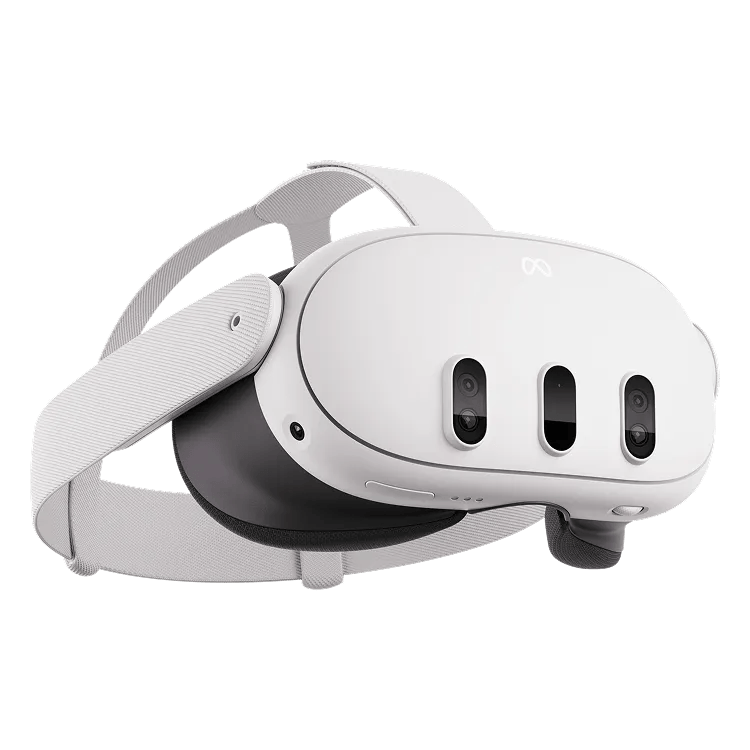
\includegraphics[width=0.55\textwidth]{images/quest3.png}
    \caption{Meta Quest 3 used as the primary Virtual Reality device in this thesis. 
    Image source: Meta \cite{metaquest3}.}
    \label{fig:quest3}
\end{figure}

These capabilities enable users to naturally interact with virtual laboratory
equipment while experiencing an immersive learning environment. The Meta Quest 3
therefore served as the primary VR platform for testing the WebXR functionality
of the developed system..

Table~\ref{tab:target_platforms} summarizes the primary hardware and software platforms supported by the proposed system.

\begin{table}[htbp]
\centering
\caption{Target hardware and software platforms}
\label{tab:target_platforms}

\renewcommand{\arraystretch}{1.3}

\begin{tabular}{p{4cm}p{9cm}}
\hline
\textbf{Component} & \textbf{Target Platform} \\
\hline

VR Headset &
Meta Quest 3 \\

Desktop Access &
Windows, Linux, or macOS computers \\

Web Browser &
Modern WebXR-compatible browsers (e.g., Meta Quest Browser, Google Chrome, Microsoft Edge) \\

Input Devices &
VR controllers, keyboard, and mouse \\

Network &
Stable Internet connection for multi-user collaboration \\

Deployment &
Browser-based application hosted on a web server \\

\hline
\end{tabular}
\end{table}
\FloatBarrier

\section{Overall Virtual Laboratory Concept}

The proposed system is designed as a browser-based immersive virtual laboratory
for interactive physics experimentation. Rather than reproducing a traditional
laboratory exactly, the environment provides a simplified virtual space in
which users can navigate between different experiment areas and interact with
physics apparatus in both desktop and immersive VR modes. The laboratory is
intended to support both individual exploration and collaborative interaction
within a shared virtual environment.

The implemented environment contains dedicated areas for the two physics
experiments developed in this thesis: the Convex Lens experiment and the
Stern--Gerlach experiment. Each experiment is placed in its own virtual area
and provides the interactive objects, controls, and visual feedback required
for the corresponding physical model. Users can move between these areas
within the same virtual environment without leaving the application.

The Convex Lens experiment represents a geometrical-optics scenario in which
users can manipulate experimental components and observe changes in image
formation and focus. The Stern--Gerlach experiment represents a quantum-physics
scenario in which users can interact with the experimental setup and observe
the corresponding measurement outcomes. The inclusion of these two experiments
demonstrates that the same virtual laboratory framework can support different
forms of physics interaction and simulation.

In addition to the implemented experiment areas, the environment contains an
AI-oriented room that was intended as a basis for exploring future
AI-assisted learning functionality. This part of the environment remains
experimental and is not considered a fully implemented component of the
system evaluated in this thesis. It is therefore treated as a prototype area
rather than as part of the core functionality.

The virtual laboratory supports both desktop and immersive VR access. Desktop
users can navigate and interact using conventional keyboard and mouse input,
whereas VR users can use motion controllers within a WebXR-compatible headset.
Regardless of the access method, connected participants share the same virtual
environment and can observe one another through avatar representations,
interact with synchronized experiment objects, and communicate through the
implemented voice communication functionality.

The overall concept is intentionally modular. Additional physics experiments
can be introduced as new experiment modules while reusing the existing
navigation, WebXR, multiplayer, and communication infrastructure. This allows
the virtual laboratory to be extended without requiring fundamental changes
to the common system architecture.

\section{User Interaction Concept}

The proposed virtual laboratory is designed to provide an intuitive and natural interaction model that enables users to focus on learning rather than on operating the system. The interaction concept is based on familiar Virtual Reality (VR) interaction techniques while also supporting conventional desktop input devices to ensure accessibility for users without VR hardware.

Upon entering the virtual laboratory, users are represented by avatars within the shared virtual environment. These avatars allow participants to observe the positions and movements of other users, thereby increasing social presence and supporting collaborative learning activities. Multiple users can occupy the same laboratory session simultaneously and interact with shared experimental equipment.

Navigation within the virtual laboratory is designed to be straightforward and consistent across different access platforms. Desktop users navigate using standard keyboard and mouse controls, whereas VR users move naturally within the immersive environment using handheld motion controllers. The virtual laboratory is organized into clearly separated areas, allowing users to move between the classroom, laboratory, and other educational spaces with minimal effort.

Interaction with experimental equipment follows a direct manipulation
approach. In VR, users can select, grab, move, and release interactive objects
using the Meta Quest Touch Plus controllers. Desktop users interact with
corresponding objects using mouse and keyboard input. Manipulation of
experimental components can modify relevant parameters of the underlying
experiment, with the resulting changes represented visually within the virtual
environment. Figure~\ref{fig:quest_controllers} shows the Meta Quest Touch Plus controllers
used for interaction during development and evaluation.

\begin{figure}[htbp]
    \centering
    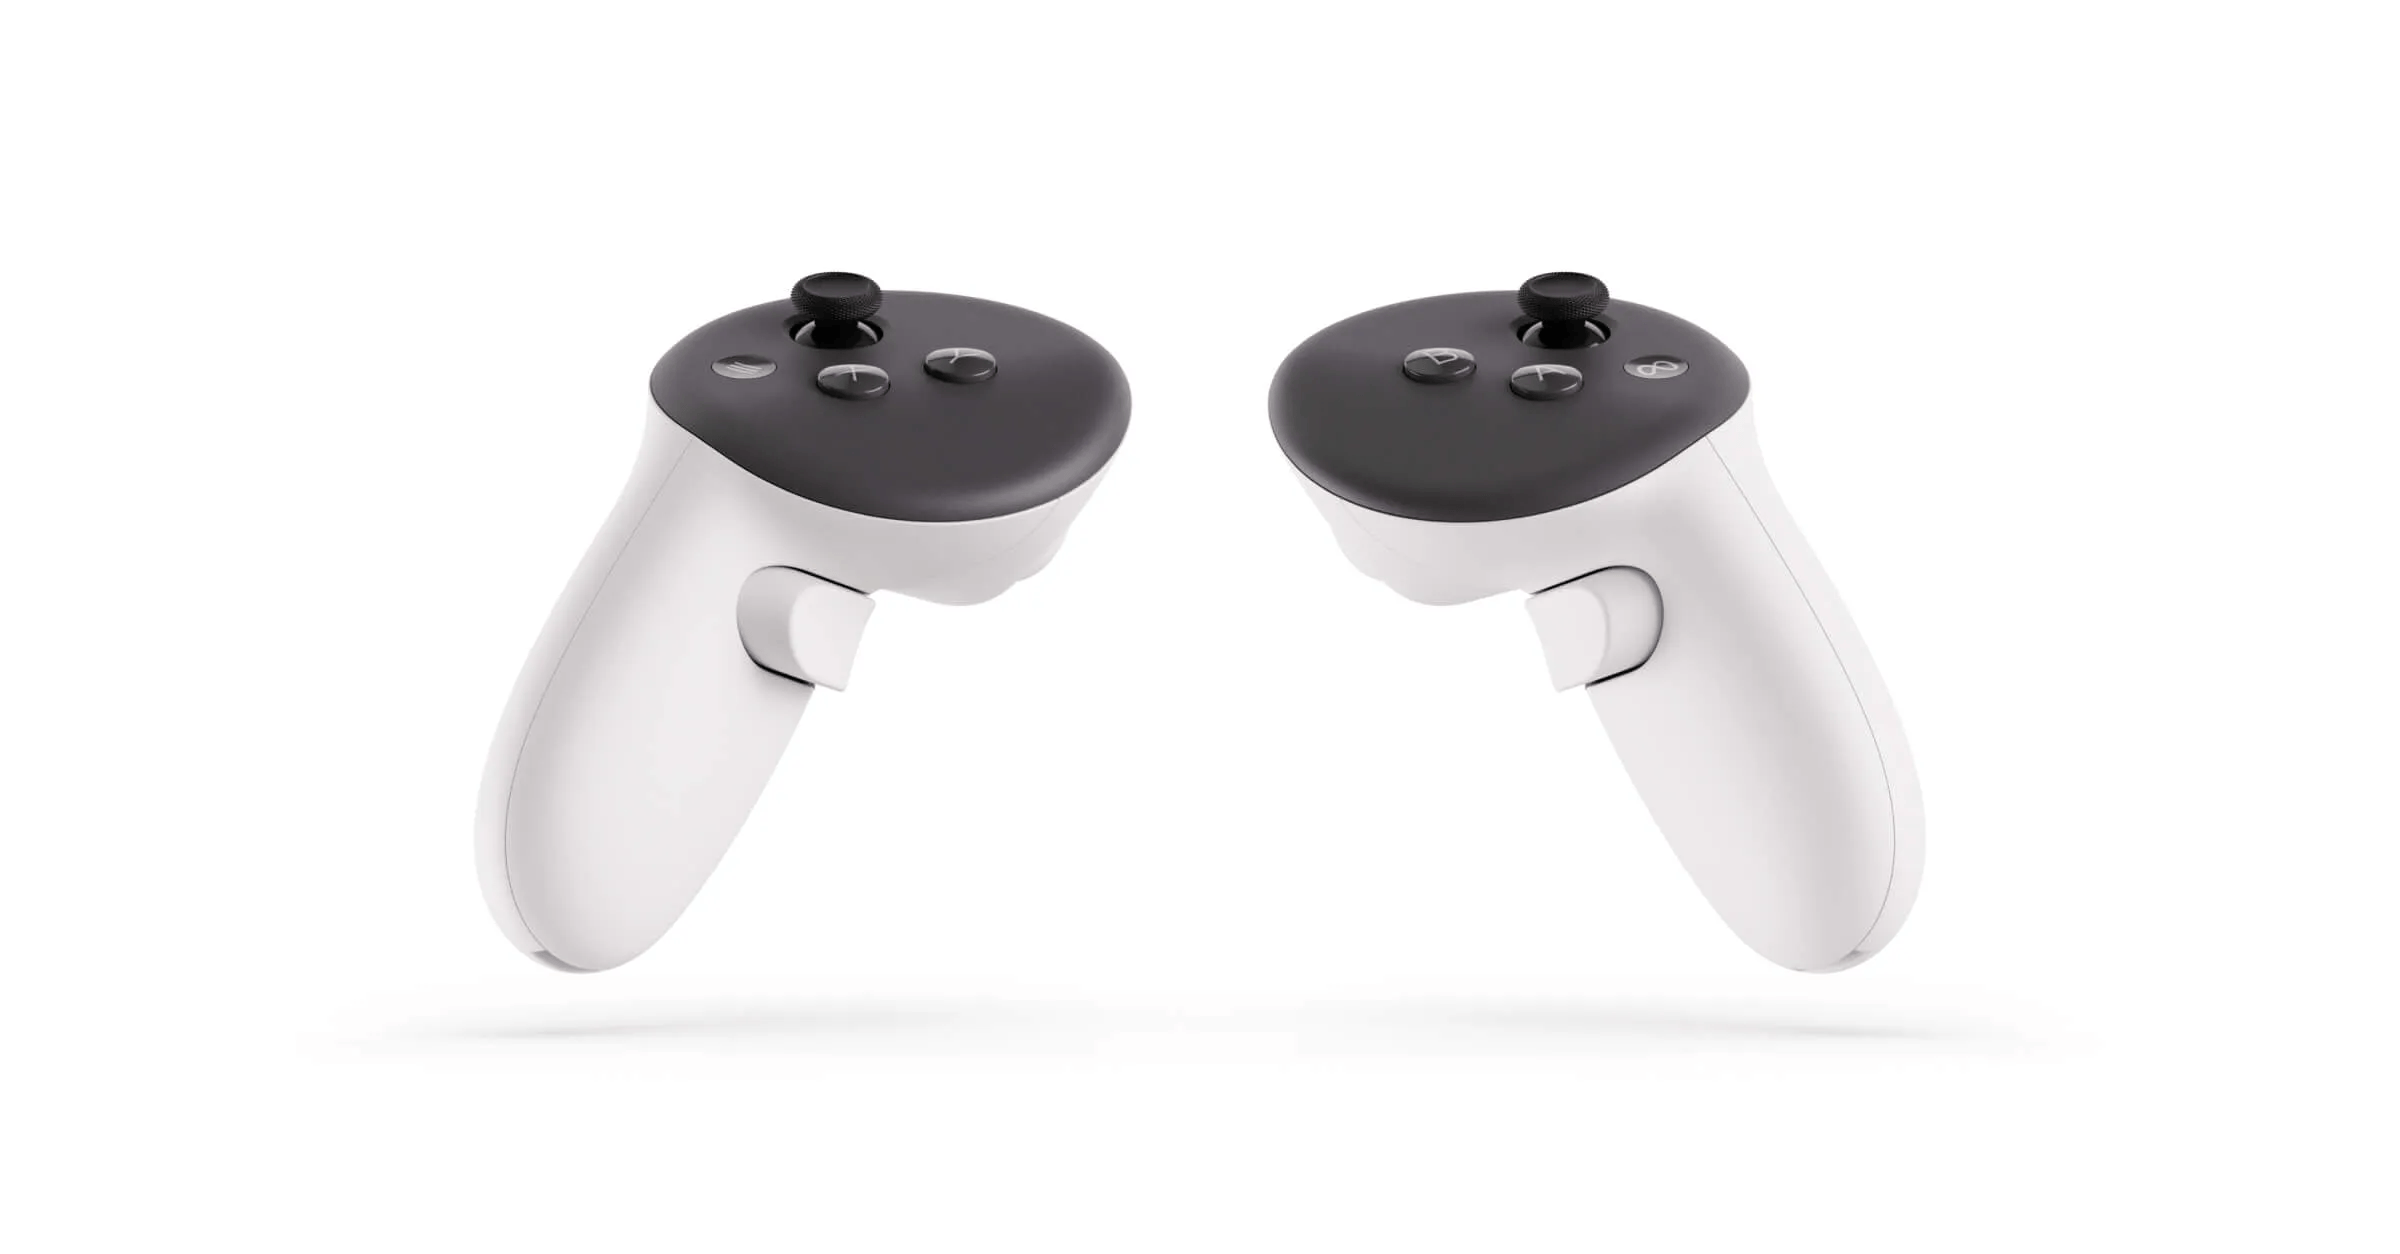
\includegraphics[width=0.55\textwidth]{images/controllers.png}
    \caption{Meta Quest  controllers. Source: Meta \cite{metaquestcontrollers}.}
    \label{fig:quest_controllers}
\end{figure}

The system also supports collaborative interaction by synchronizing user actions across all connected participants. When one user manipulates an experimental object, the corresponding changes are reflected in real time for all other users within the same laboratory session. This shared interaction enables collaborative experimentation, instructor demonstrations, and group discussions that resemble traditional laboratory activities.

To minimize the learning curve, the graphical user interface is intentionally kept simple and unobtrusive. Menus and interface elements provide only the controls required for navigation, experiment selection, and entering or exiting VR mode. The majority of user interaction occurs directly within the virtual environment, reducing distractions and preserving immersion.

Overall, the interaction concept aims to provide an accessible, immersive, and collaborative user experience that supports effective learning while remaining sufficiently flexible to accommodate future experiments and additional interaction techniques.